\fontsize{13}{14}\selectfont
\chapter{Thiết kế hệ thống}
\newpage
\section{Hardware}
	\subsection{Tổng quan hệ thống}
	\begin{figure}[H]
		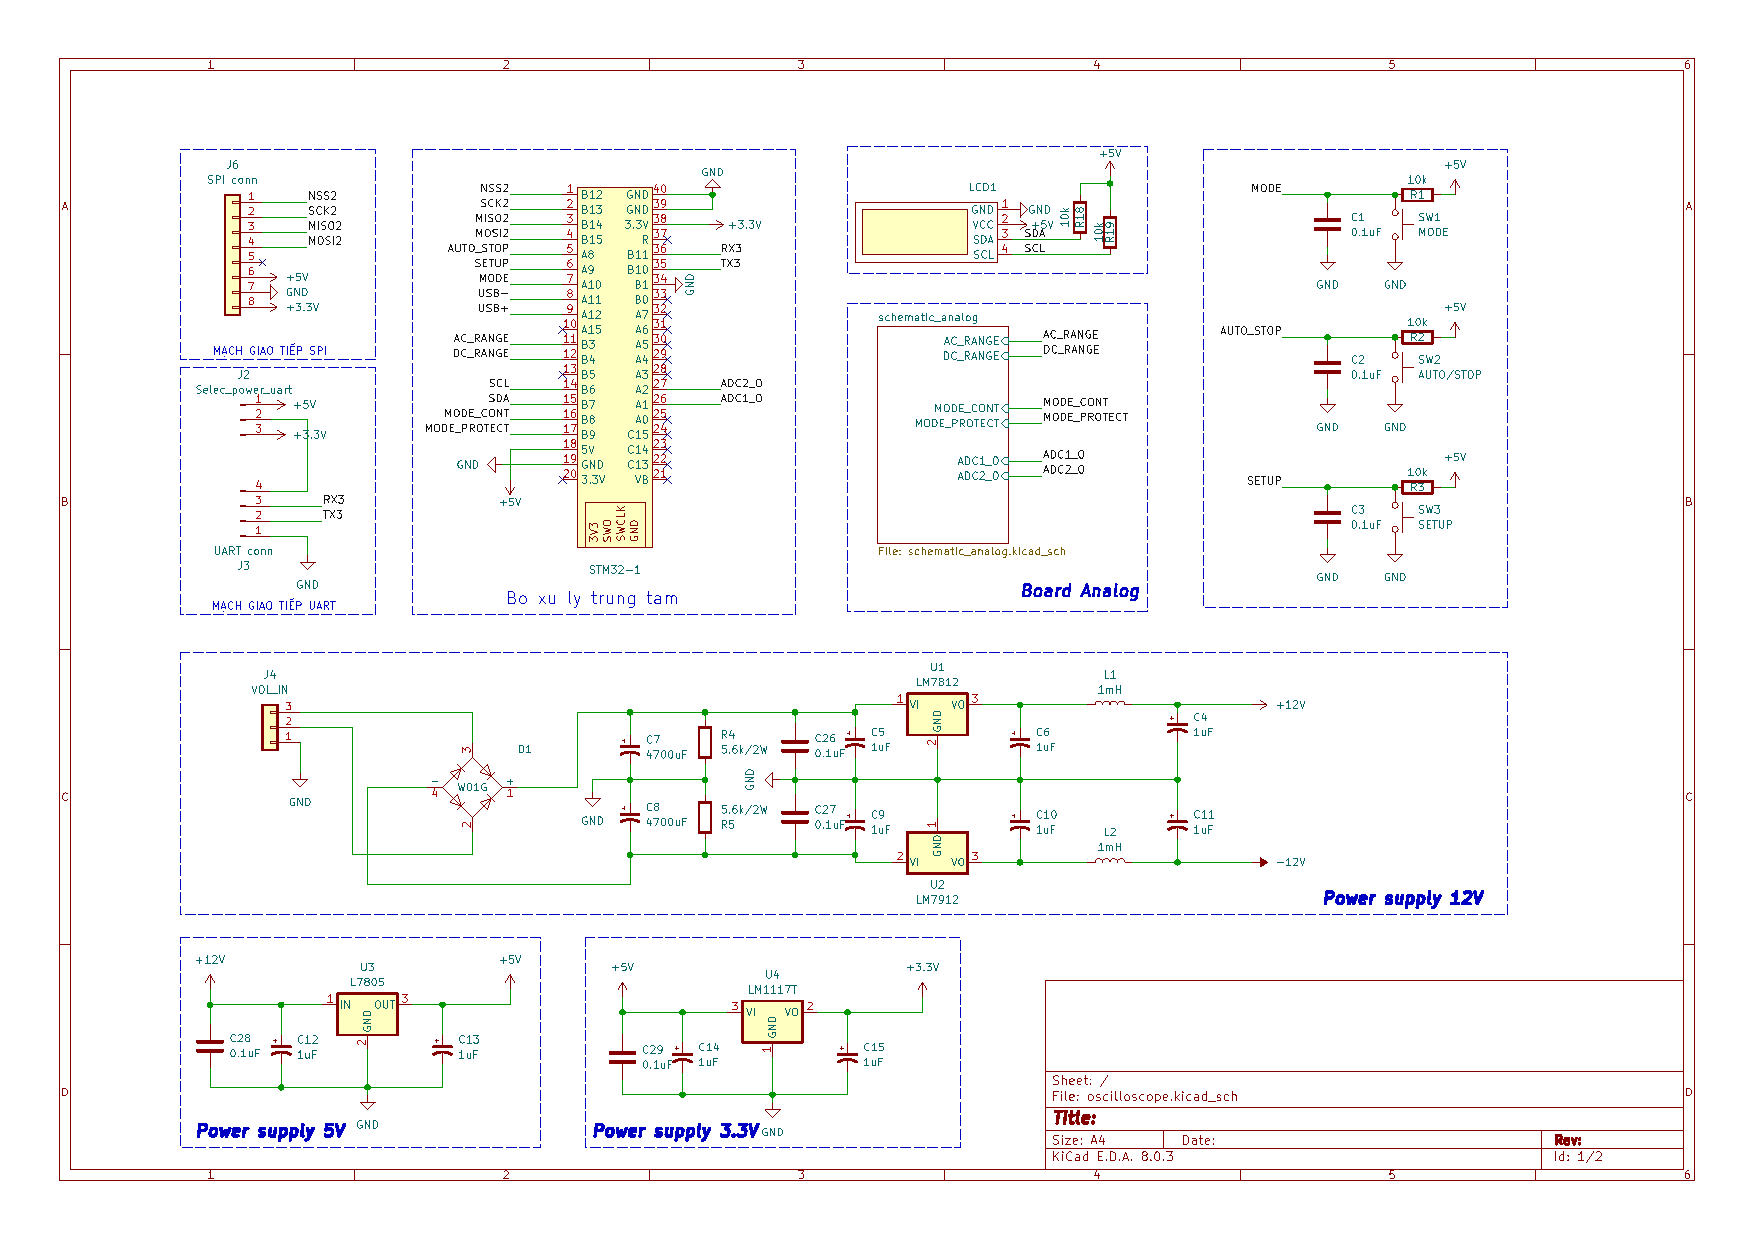
\includegraphics[width=\linewidth]{./picture/over_hardware.pdf}
		\caption{Tổng quan phần cứng của hệ thống}
		\label{over_hardware}
	\end{figure}
	
	\subsection{Khối nguồn}
	
	Sử dụng nguồn cấp cho mạch là $220$VAc, chuyển đổi về nguồn $\pm 12$VDc, $+5$VDc và $+3.3$VDc.
	
	\subsubsection{Mạch hỗ trợ cho ra nguồn $\pm 12$VDc}
	
	\begin{figure}[H]
		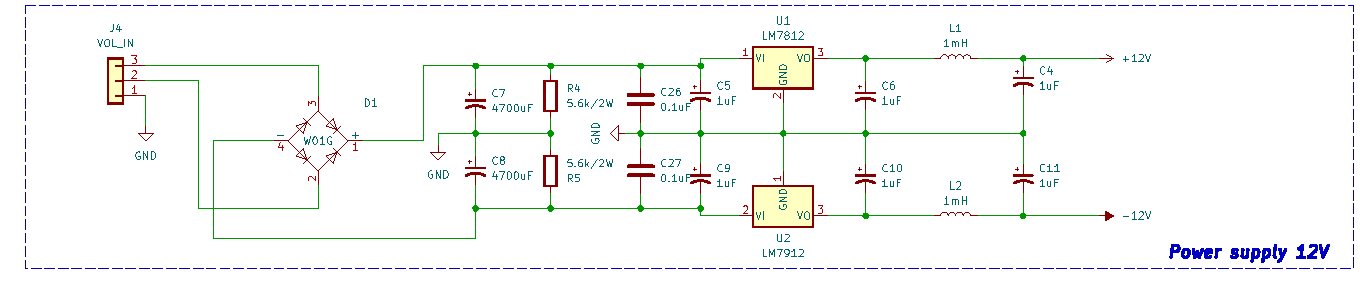
\includegraphics[width=\linewidth]{./picture/power_supply.pdf}
		\caption{Khối nguồn cung cấp $\pm12V$}
		\label{power_supply_hardware}
	\end{figure}
	
	Mạch sử dụng:
	
	\begin{itemize}[label= - ]
		\item \textbf{Biến áp:}
		
		\begin{minipage}{0.3\linewidth}
			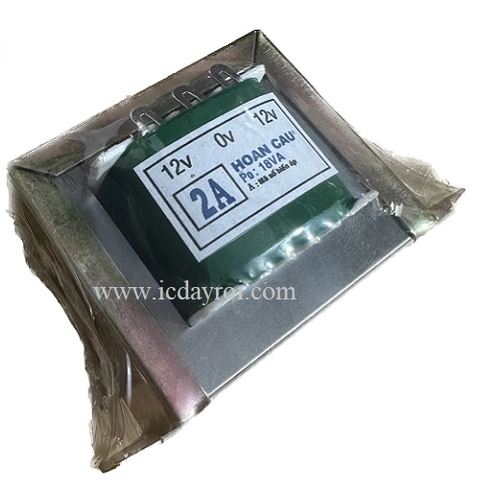
\includegraphics[width=\linewidth]{./picture/transformer_12V.png}
		\end{minipage}
		\begin{minipage}{0.7\linewidth}		
			\begin{itemize}[label = -]
				\item Điện áp vào: $0V - 110V - 220V$
				\item Điện áp ra: $12V - 0V - 12V$
				\item Dòng điện ra: $2A$
				\item Kích thước: $63.5 \times 53 \times 26$ mm
				\item Khoảng cách 2 lỗ cố định biến áp: $80$mm
				\item Khối lượng: $600$g
			\end{itemize}
		\end{minipage}
		\item \textbf{KBP206 Diode cầu chỉnh lưu:}
		
		\begin{minipage}{0.3\linewidth}
			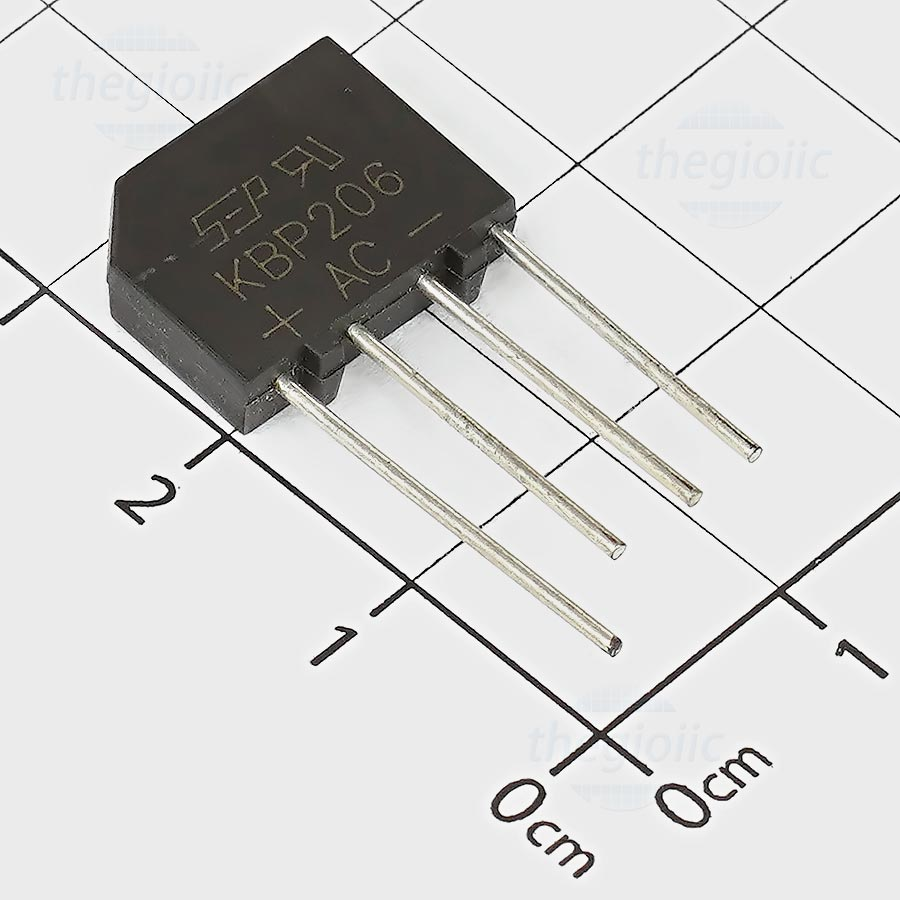
\includegraphics[width=\linewidth]{./picture/bright_diode.png}
		\end{minipage}
		\begin{minipage}{0.7\linewidth}
			\begin{itemize}[label = -]
				\item Loại Diode: 1 pha
				\item Điện áp ngược cực đại: $600V$
				\item Dòng điện chỉnh lưu trung bình: $2A$
				\item Điện áp Forward max: $1.1V-2A$
				\item Dòng rò ngược: $10\mu A - 600V$
				\item Nhiệt độ hoạt động: $-55^{\circ}C \sim 150^{\circ}C$
				\item Kiểu đóng gói: 4-SIP, KBP
			\end{itemize}
		\end{minipage}
		\item \textbf{LM7912}
		
		\begin{minipage}{0.3\linewidth}
			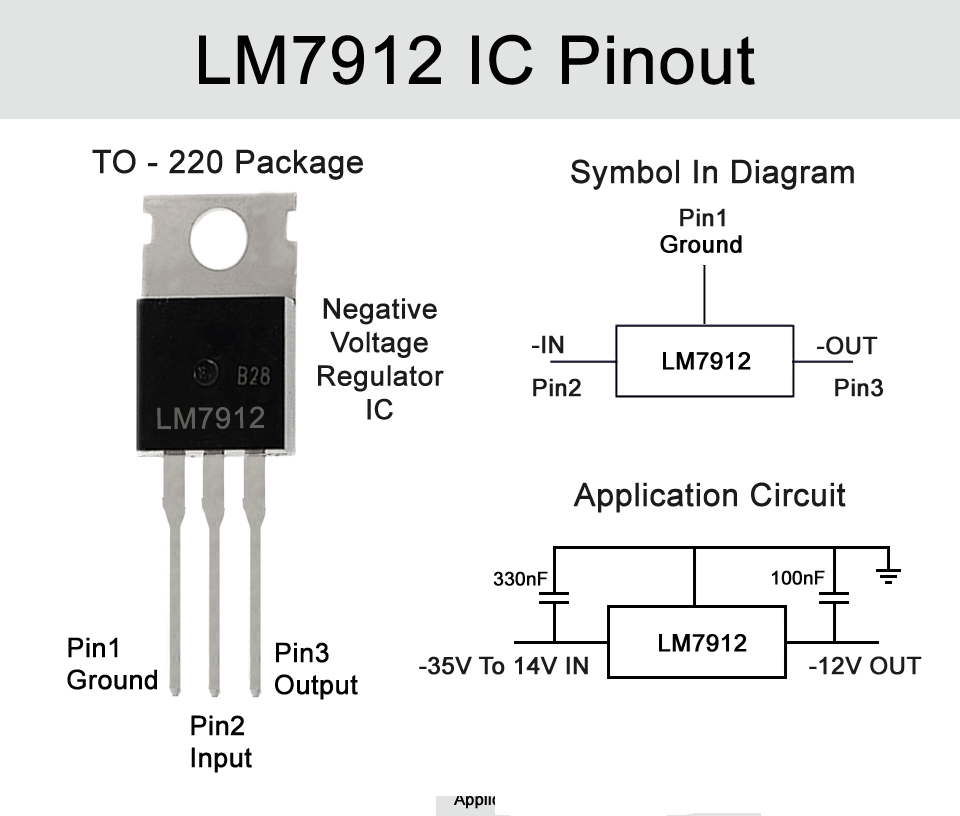
\includegraphics[width=\linewidth]{./picture/lm7912.png}
		\end{minipage}
		\begin{minipage}{0.7\linewidth}
			\begin{itemize}[label = -]
				\item Điện áp đầu vào cực đại: $-35V$
				\item Điện áp đầu ra: $-12V$
				\item Nhiệt độ hoạt động: $-40^{\circ}C \sim 155^{\circ}C$
				\item Kiểu đóng gói: TO-220
			\end{itemize}
		\end{minipage}
		\item \textbf{LM7812}
		
		\begin{minipage}{0.3\linewidth}
			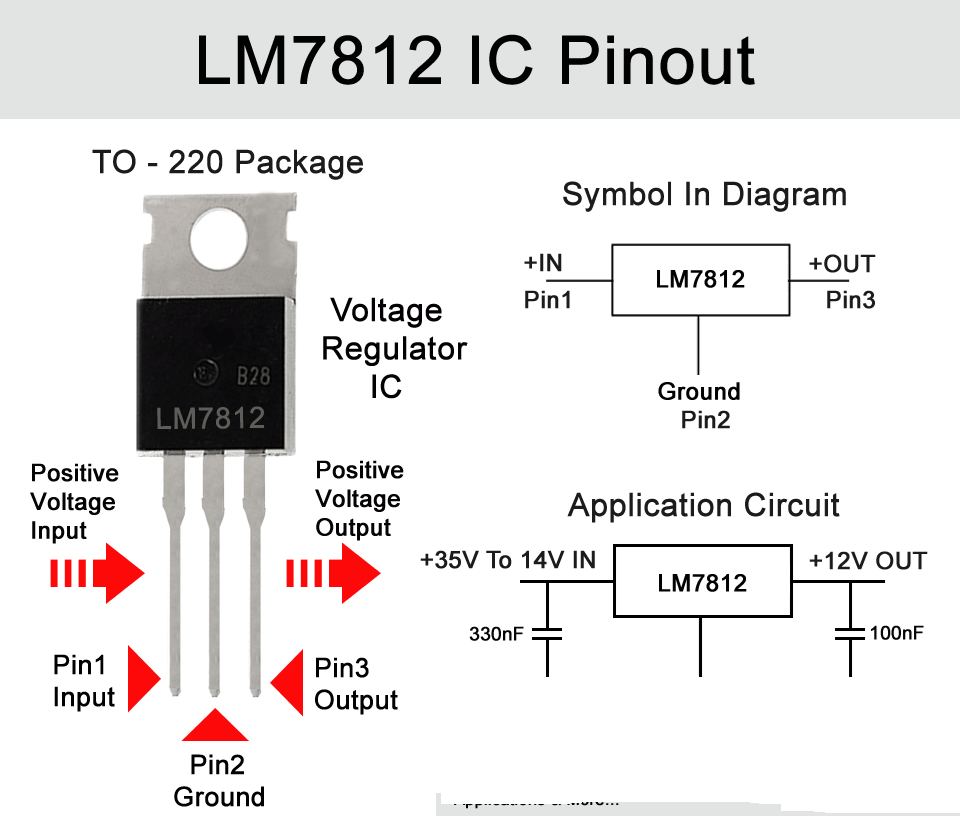
\includegraphics[width=\linewidth]{./picture/lm7812.png}
		\end{minipage}
		\begin{minipage}{0.7\linewidth}
			\begin{itemize}[label = -]
				\item Điện áp đầu vào cực đại: $35V$
				\item Điện áp đầu ra: $12V$
				\item Nhiệt độ hoạt động: $0^{\circ}C \sim 125^{\circ}C$
				\item Kiểu đóng gói: TO-220
			\end{itemize}
		\end{minipage}
	\end{itemize}
	
	\subsubsection{Mạch trợ cho ra nguồn $5$VDc}
	
	\begin{figure}[H]
		\centering
		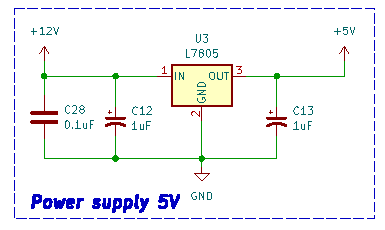
\includegraphics[width=0.7\linewidth]{./picture/power_supply_5V.pdf}
		\caption{Khối nguồn cung cấp $5V$}
		\label{power_supply_5V_hardware}
	\end{figure}
	
	\begin{itemize}[label= - ]
		\item \textbf{LM7805}
		
		\begin{minipage}{0.3\linewidth}
			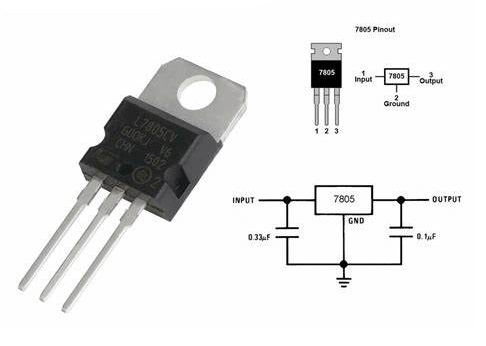
\includegraphics[width=\linewidth]{./picture/lm7805.png}
		\end{minipage}
		\begin{minipage}{0.7\linewidth}
			\begin{itemize}[label = -]
				\item Điện áp đầu vào cực đại: $35V$
				\item Điện áp đầu ra: $5V$
				\item Nhiệt độ hoạt động: $0^{\circ}C \sim 125^{\circ}C$
				\item Kiểu đóng gói: TO-220
			\end{itemize}
		\end{minipage}
	\end{itemize}
	
	\subsubsection{Mạch trợ cho ra nguồn $3.3$VDc}
	
	\begin{figure}[H]
		\centering
		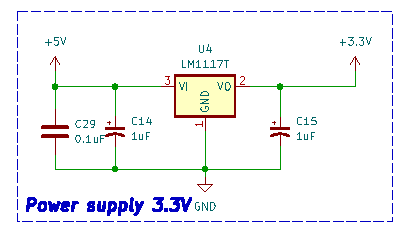
\includegraphics[width=0.7\linewidth]{./picture/power_supply_3V.pdf}
		\caption{Khối nguồn cung cấp $3.3V$}
		\label{power_supply_3.3V_hardware}
	\end{figure}
	
	\begin{itemize}[label= - ]
		\item \textbf{LM1117T}
		
		\begin{minipage}{0.3\linewidth}
			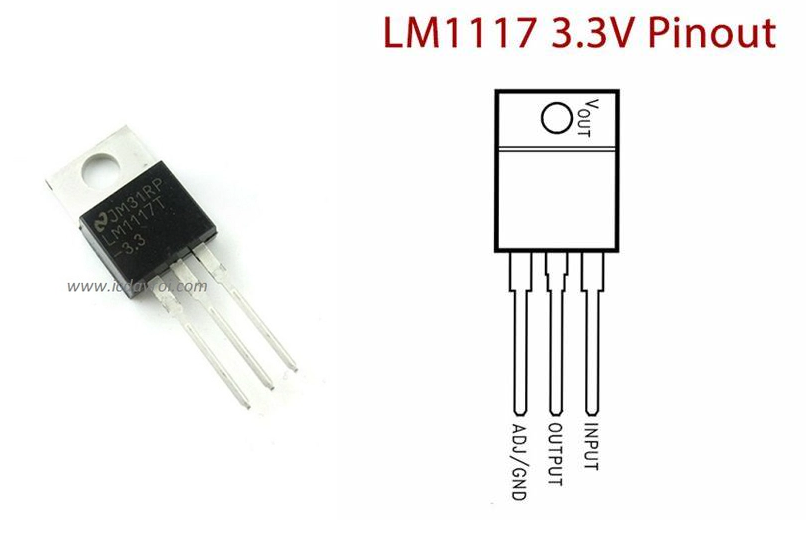
\includegraphics[width=\linewidth]{./picture/lm1117T.png}
		\end{minipage}
		\begin{minipage}{0.7\linewidth}
			\begin{itemize}[label = -]
				\item Điện áp đầu vào cực đại: $15V$
				\item Điện áp đầu ra: $3.3V$
				\item Nhiệt độ hoạt động: $0^{\circ}C \sim 125^{\circ}C$
				\item Kiểu đóng gói: TO-220
			\end{itemize}
		\end{minipage}
	\end{itemize}
	
	\subsection{Khối xử lý}
	Sử dụng STM32F103C6T8 làm chip xử lý chính.
	
	\begin{figure}[H]
		\centering
		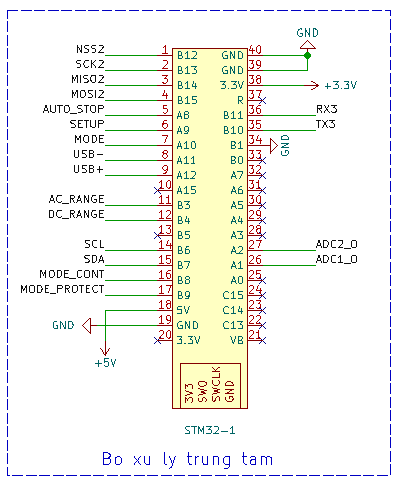
\includegraphics[width=0.7\linewidth]{./picture/main_vxl.pdf}
		\caption{Khối xử lý trung tâm}
		\label{main vxl}
	\end{figure}
	
	\subsection{Khối mạch đo tín hiệu Analog}
	
	\begin{figure}[H]
		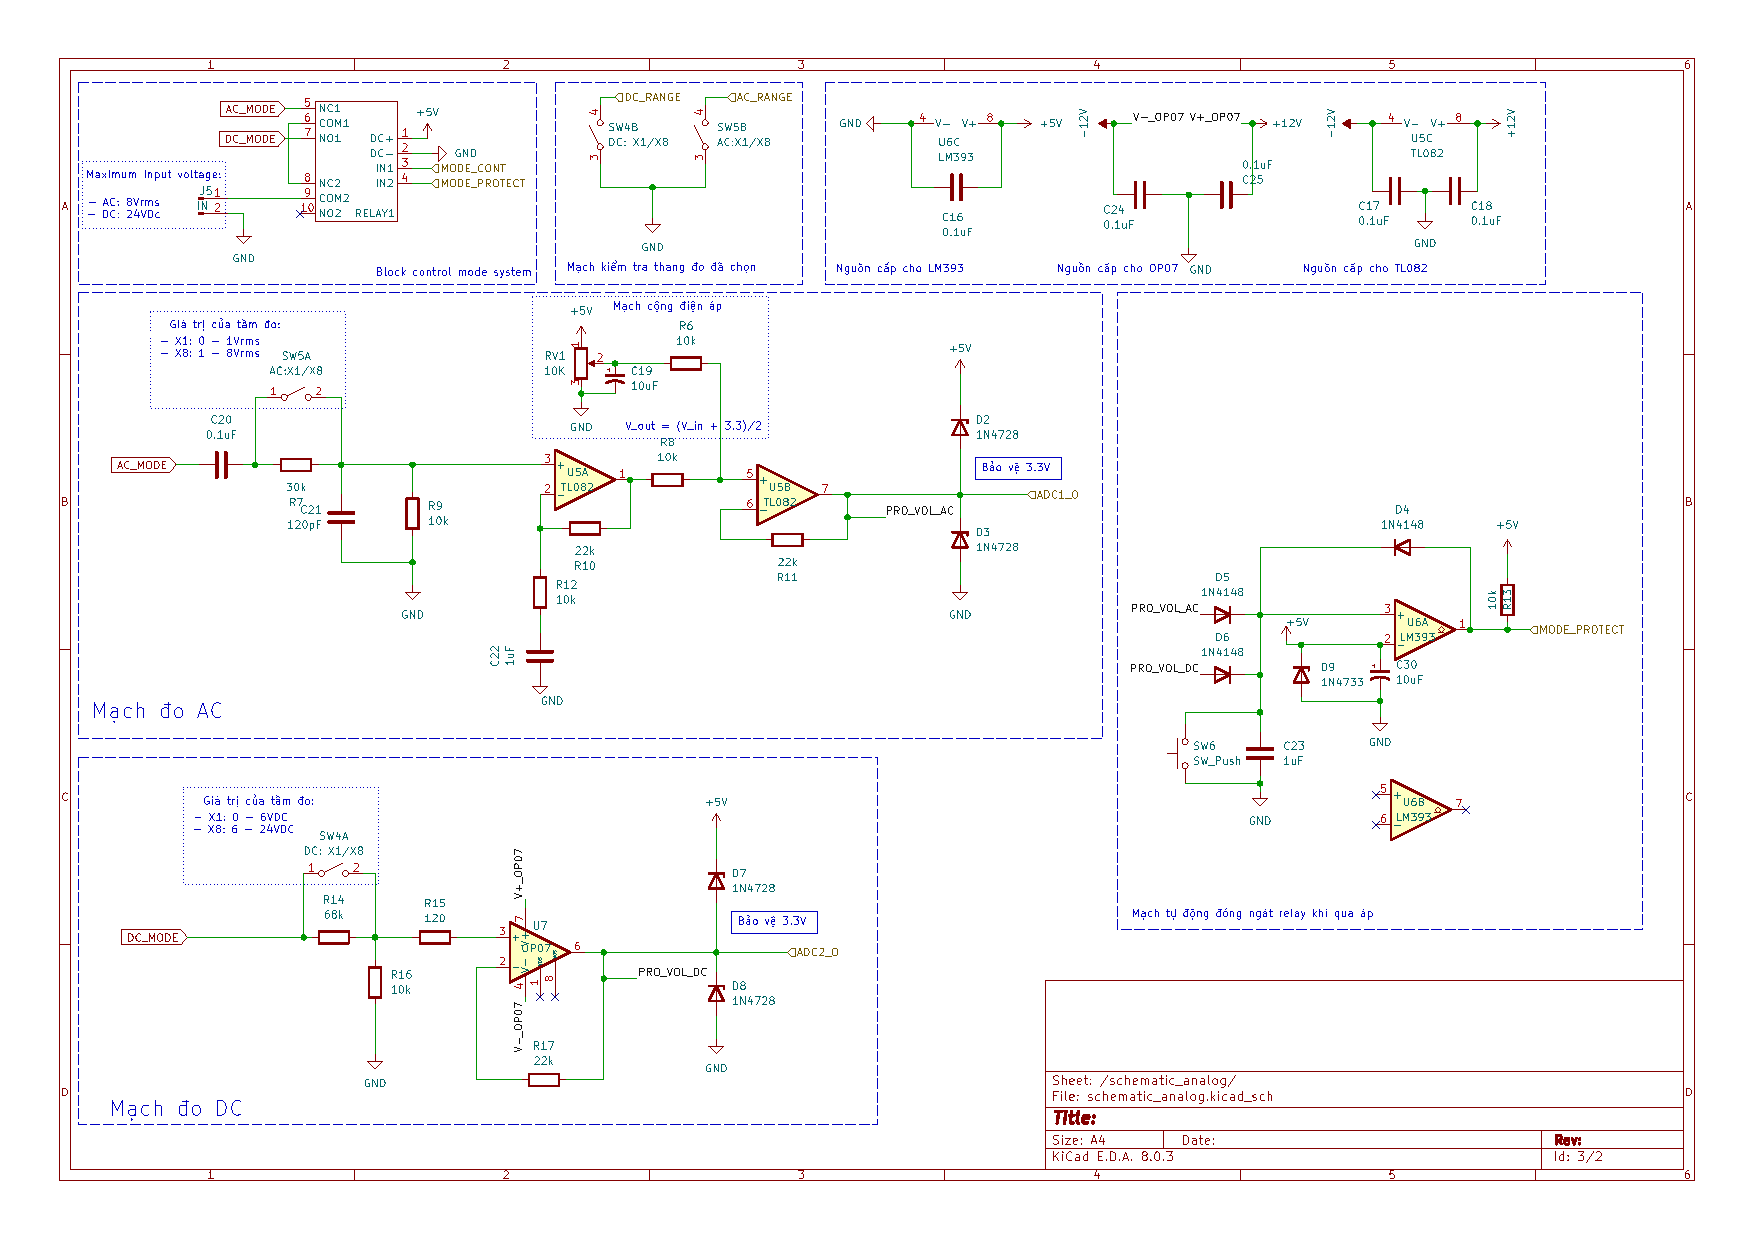
\includegraphics[width=\linewidth]{./picture/board_analog.pdf}
		\caption{Khối mạch đo tín hiệu Analog}
		\label{board analog}
	\end{figure}
	
	\subsubsection{Mạch đo AC}
	
	Ở chế độ AC có hai tầm đo chính của hệ thống là:
	
	\begin{itemize}[label=-]
		\item Tầm đo từ $0 - 1Vrms$ (X1): cho phép bộ ADC đọc tín hiệu đầu vào một cách trực tiếp không cần phải khuếch đại xuống.
		\item Tầm đo từ $1 - 8Vrms$ (X8): cho phép bộ ADC đọc được tín hiệu lớn hơn thông qua việc khuếch đại xuống tín hiệu vào đúng tầm đo của bộ ADC.
	\end{itemize}
	
	Mạch sử dụng một mạch cộng tín hiệu lên để có thể dời toàn bộ giá trị của tín hiệu đầu vào lên hết phần dương để bộ ADC của khối xử lý trung tâm có thể đọc được.
	
	Việc chọn IC để cho việc làm bộ tiền lọc tín hiệu trước khi vào bộ ADC cần phải đảm bảo các yếu tố sau đây:
	
	\begin{itemize}[label=-]
		\item \textbf{Trở kháng đầu vào cao} để không ảnh hưởng đến mạch nguồn tín hiệu AC đầu vào.
		\item \textbf{Trở kháng đầu ra thấp} để truyền tính hiệu hiệu quả đến ADC.
		\item \textbf{Độ tuyến tính cao và sai số nhỏ} để đảm bảo giá trị đầu ra phản ánh đúng với giá trị đầu vào.
		\item \textbf{Băng thông rộng} để đảm bảo đáp ứng đầy đủ tần số trong khoảng từ $20 - 20KHz$ của tín hiệu AC đầu vào.
		\item \textbf{Tốc độ đáp ứng (Slew rate) đủ lớn} tối thiểu phải là $12V/ \mu s$ để có thể đảm bảo đáp ứng đủ nhanh so với tốc độ thay đổi đột ngột của tín hiệu.
		\item \textbf{Điện áp offset đầu vào giữa hai chân cần nhỏ} tối đa là $5mV$ để có thể đảm bảo giá trị đầu vào không sai số quá nhiều (không vượt quá $20\%$).
		\item \textbf{Nguồn cấp ổn định và các có thể hoạt động ở chế độ dual} để phù hợp để có thể đo được giá trị AC.
	\end{itemize}
	
	Với các yêu cầu trên có các IC sau đây phù hợp:
	
		\begin{table}[H]
			\centering
			\begin{tabular}{|>{\centering\arraybackslash}p{0.1\linewidth}|p{0.8\linewidth}|}
				\hline
				\textbf{IC} & \textbf{Thông số kỹ thuật} \\ \hline
				OPA2134     & \begin{itemize}
					\item Trở kháng đầu vào: Rất cao ($10^{13} \Omega$).
					\item Băng thông: 8MHz (áp dụng tốt cho tín hiệu AC).
					\item Slew Rate: $20V/\mu s$ (đáp ứng nhanh).
					\item Điện áp offset: $<2mV$ (độ chính xác cao). 		
				\end{itemize} \\ \hline
				TL072       & \begin{itemize}
					\item Trở kháng đầu vào: Rất cao ($10^{12} \Omega$).
					\item Băng thông: 3MHz.
					\item Slew Rate: $13V/\mu s$.
					\item Điện áp offset: $3mV$. 		
				\end{itemize} \\ \hline
				TL082       & \begin{itemize}
					\item Trở kháng đầu vào: Rất cao ($10^{12} \Omega$).
					\item Băng thông: 3MHz.
					\item Slew Rate: $13V/\mu s$.
					\item Điện áp offset: $5mV$. 		
				\end{itemize} \\ \hline
			\end{tabular}
			
			\caption{Bảng thông số kỹ thuật các IC cho mạch đo AC.}
			\label{tab:ic_AC}
		\end{table}
		
		Với những thông số kỹ thuật trên thì lựa chọn OPA2134 là lựa chọn hợp lý. Tuy nhiên, với vấn đề giá cả và khả năng dễ mua trên thị trường thì lựa chọn TL072 là lựa chọn hợp lý hơn mà vẫn đáp ứng đủ các như cầu trên.
		
	\subsubsection{Mạch đo DC}
	
	Ở chế độ DC có hai tầm đo chính của hệ thống là:
	
	\begin{itemize}[label=-]
		\item Tầm đo từ $0 - 3VDc$ (X1): cho phép bộ ADC đọc tín hiệu đầu vào một cách trực tiếp không cần phải khuếch đại xuống.
		\item Tầm đo từ $3 - 24VDc$ (X8): cho phép bộ ADC đọc được tín hiệu lớn hơn thông qua việc khuếch đại xuống tín hiệu vào đúng tầm đo của bộ ADC.
	\end{itemize}
	
	Việc chọn IC phù hợp cho việc đo tín hiệu DC cần phải đáp ứng các yêu cầu sau:
	
	\begin{itemize}[label = -]
		\item \textbf{Trở kháng đầu vào cao} để không ảnh hưởng đến mạch nguồn tín hiệu DC đầu vào.
		\item \textbf{Trở kháng đầu ra thấp} để truyền tính hiệu hiệu quả đến ADC.
		\item \textbf{Độ tuyến tính cao và sai số nhỏ} để đảm bảo giá trị đầu ra phản ánh đúng với giá trị đầu vào.
		\item \textbf{Điện áp offset đầu vào giữa hai chân cần nhỏ và có thể điều chỉnh được điện áp offset} tối đa là $5mV$ để có thể đảm bảo giá trị đầu vào không sai số quá nhiều (không vượt quá $20\%$).
		\item \textbf{Nguồn cấp ổn định} để phù hợp để có thể đo được giá trị DC.
	\end{itemize}
	
	Với các yêu cầu trên có các IC phù hợp sau đây:
	
	\begin{table}[H]
		\centering
		\begin{tabular}{|>{\centering\arraybackslash}p{0.1\linewidth}|p{0.8\linewidth}|}
			\hline
			\textbf{IC} & \textbf{Thông số kỹ thuật} \\ \hline
			OP70     & \begin{itemize}
				\item Băng thông: 600kHz.
				\item Slew Rate: $0.3V/\mu s$.
				\item Điện áp offset: $60\mu V$.
					   \end{itemize}  \\ \hline
			TL072     & \begin{itemize}
				\item Băng thông: 3MHz.
				\item Slew Rate: $13V/\mu s$.
				\item Điện áp offset: $3mV$.
					   \end{itemize} \\ \hline
			LF356     & \begin{itemize}
				\item Băng thông: 5MHz.
				\item Slew Rate: $12V/\mu s$.
				\item Điện áp offset: $2mV$.
			\end{itemize} \\ \hline
		\end{tabular}
		
		\caption{Bảng thông số kỹ thuật các IC cho mạch đo DC.}
		\label{tab:ic_DC}
	\end{table}
	
	Với những thông số kỹ thuật trên thì lựa chọn hợp lý nhất là OP07. Vì OP07 đáp ứng hết các yêu cầu và tương đối dễ mua trên thị và giá thành rẻ.
	
	\subsubsection{Mạch bảo vệ khi quá áp đầu vào ADC}
	
	\begin{itemize}[label=-]
		\item Mạch xén áp sử dụng Zener ổn áp
	
		\begin{figure}[H]
			\centering
			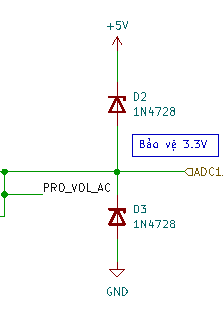
\includegraphics[width=0.5\linewidth]{./picture/protect_ADC.pdf}
			\caption{Mạch xén áp bảo vệ 3.3V}
			\label{t_mach xen ap bao ve}
		\end{figure}
	
	Nếu điện áp ở ngõ vào DC lớn hơn $3.3V$ thì zener 1N4728 sẽ ghim điện áp ở mức $3.3V$ để đảm bảo an toàn cho bộ xử lý trung tâm.
	
	\item Mạch bảo vệ bằng mạch so sánh
	
	\begin{figure}[H]
		\centering
		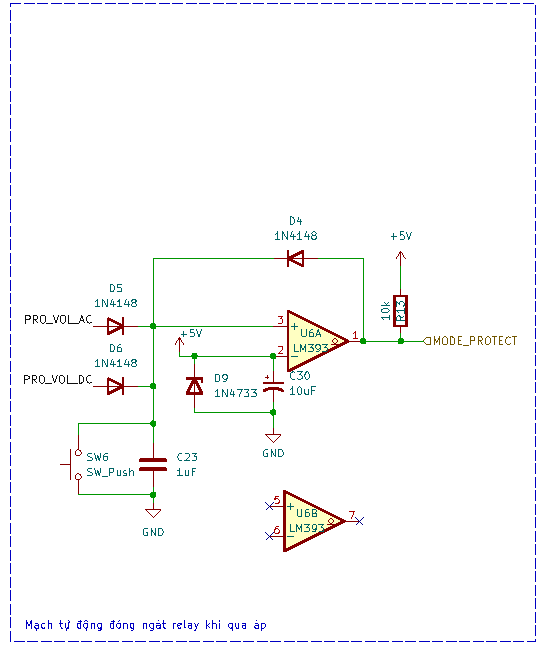
\includegraphics[width=0.7\linewidth]{./picture/pro_compere.pdf}
		\caption{Mạch bảo vệ đóng ngắt khi quá áp}
		\label{t_mach bao ve dong ngat khi qua ap}
	\end{figure}
	
	Mạch sử dụng mạch so sánh để thực hiện chức năng bảo vệ, nếu ngõ vào chân 3 của LM393 lớn hơn điện áp so sanh ở đây là 5V thì ở chân ngõ ra 1 sẽ được kéo xuống GND để bật relay giúp ngắt tín hiệu đầu vào que đo ra khỏi mạch đo.
	\end{itemize}
	
	\subsection{Các thành phần khác}
	
	\begin{itemize}[label=-]
		\item \textbf{LCD 16x2 và module I2C PCF8574:}
		
		\begin{minipage}{0.3\linewidth}
			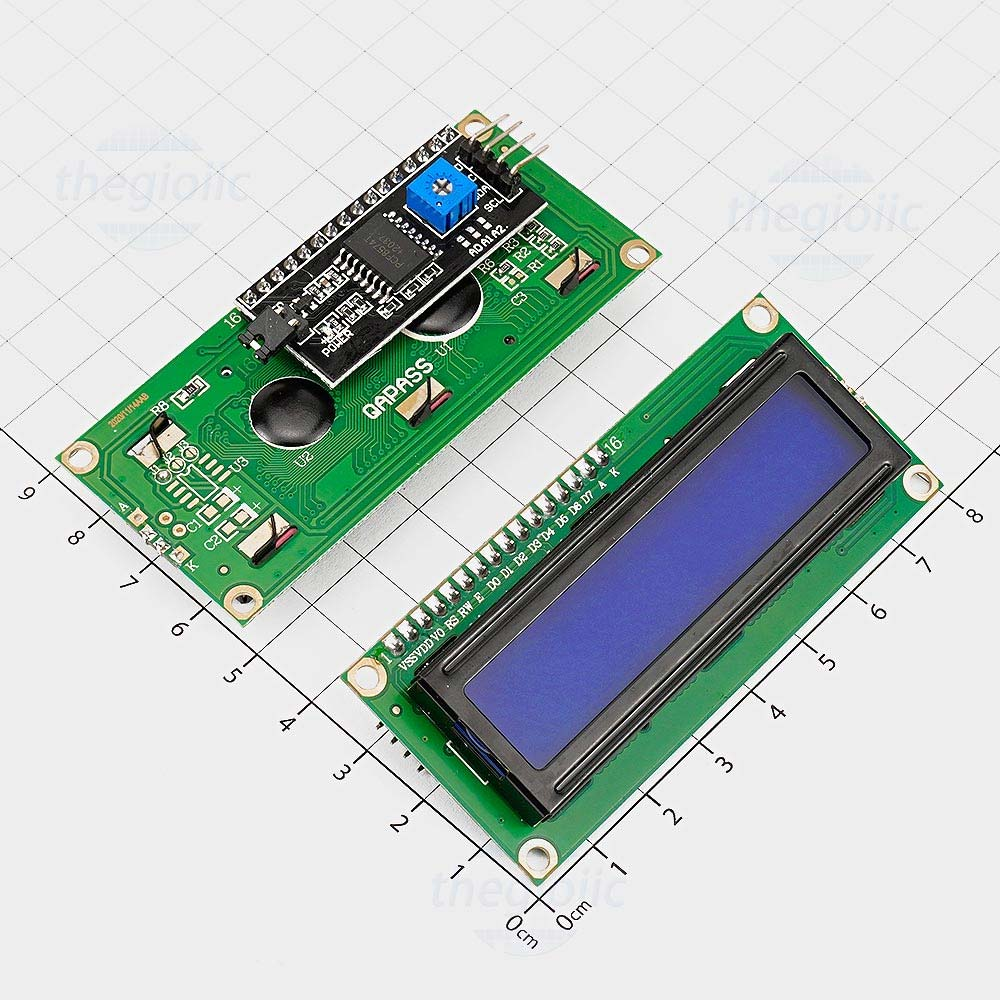
\includegraphics[width=\linewidth]{./picture/lcd.png}
		\end{minipage}
		\begin{minipage}{0.7\linewidth}		
			\begin{itemize}[label = -]
				\item LCD STN độ tương phản cao 16x2
				\item Điện áp hoạt động: $+5DC$
				\item Ký tự 5x8 dot
				\item IC điều khiển HD44780 hoặc tương đương
				\item Module: $80 \times 36 \times 13.5$mm
			\end{itemize}
		\end{minipage}
		\item \textbf{Module Relay 5VDc 2 kênh:}
		
		\begin{minipage}{0.3\linewidth}
			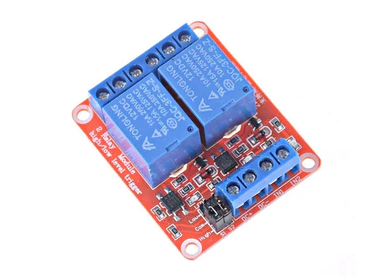
\includegraphics[width=\linewidth]{./picture/relay_2kenh.png}
		\end{minipage}
		\begin{minipage}{0.7\linewidth}		
			\begin{itemize}[label = -]
				\item Nguồn đầu vào: $5VDc$
				\item Điện áp hoạt động: $+5DC$
				\item Jump H/L level trigger: thiết lập mức điều khiển relay. Có 2 mức : HIGH / LOW
				\item COM: Tiếp điểm relay 220V 10A
				\item NO: chân thường mở
				\item NC: chân thường đóng
			\end{itemize}
		\end{minipage}
	\end{itemize}
	
\section{Firmware}

\subsection{Lưu đồ giải thuật của hệ thống}

\begin{figure}[H]
	\centering
	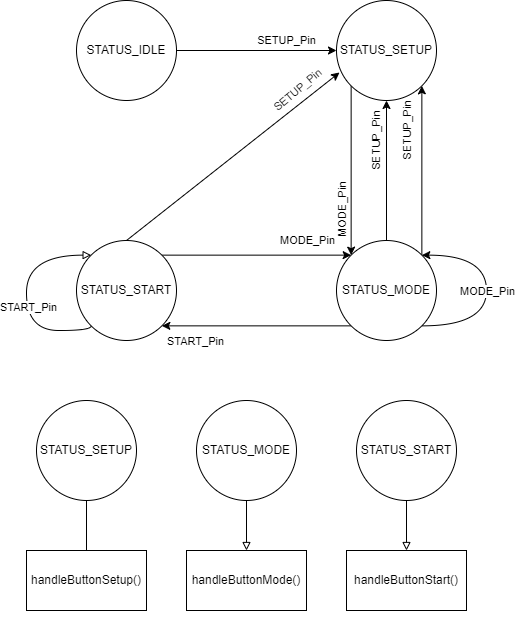
\includegraphics[width=0.7\linewidth]{./diagram/fsm.drawio.png}
	\caption{FSM của hệ thống}
	\label{f_fsm system}
\end{figure}

Hệ thống hoạt động chủ yếu ở 4 trạng thái:

\begin{itemize}[label = -]
	\item \texttt{STATUS\_IDLE}: là trạng thái mà hệ thống ở trạng thái khởi động.
	\item \texttt{STATUS\_SETUP}: là trạng thái mà đưa trạng thái về ban đầu và khởi động các hàm hoạt động của hệ thống như khởi động các hàm ngắt, khởi động LCD, khởi động các giao thức giao tiếp.
	\item \texttt{STATUS\_MODE}: là trạng thái định dạng hệ thống sẽ hoạt động động ở chế độ đo AC/DC.
	\item \texttt{STATUS\_START}: là trạng thái hoạt động của hệ thống khi đã được định nghĩa từ trước, cho phép hệ thống tiếp tục hoạt động hay là dừng hệ thống lại.
\end{itemize}

\begin{figure}[H]
	\centering
	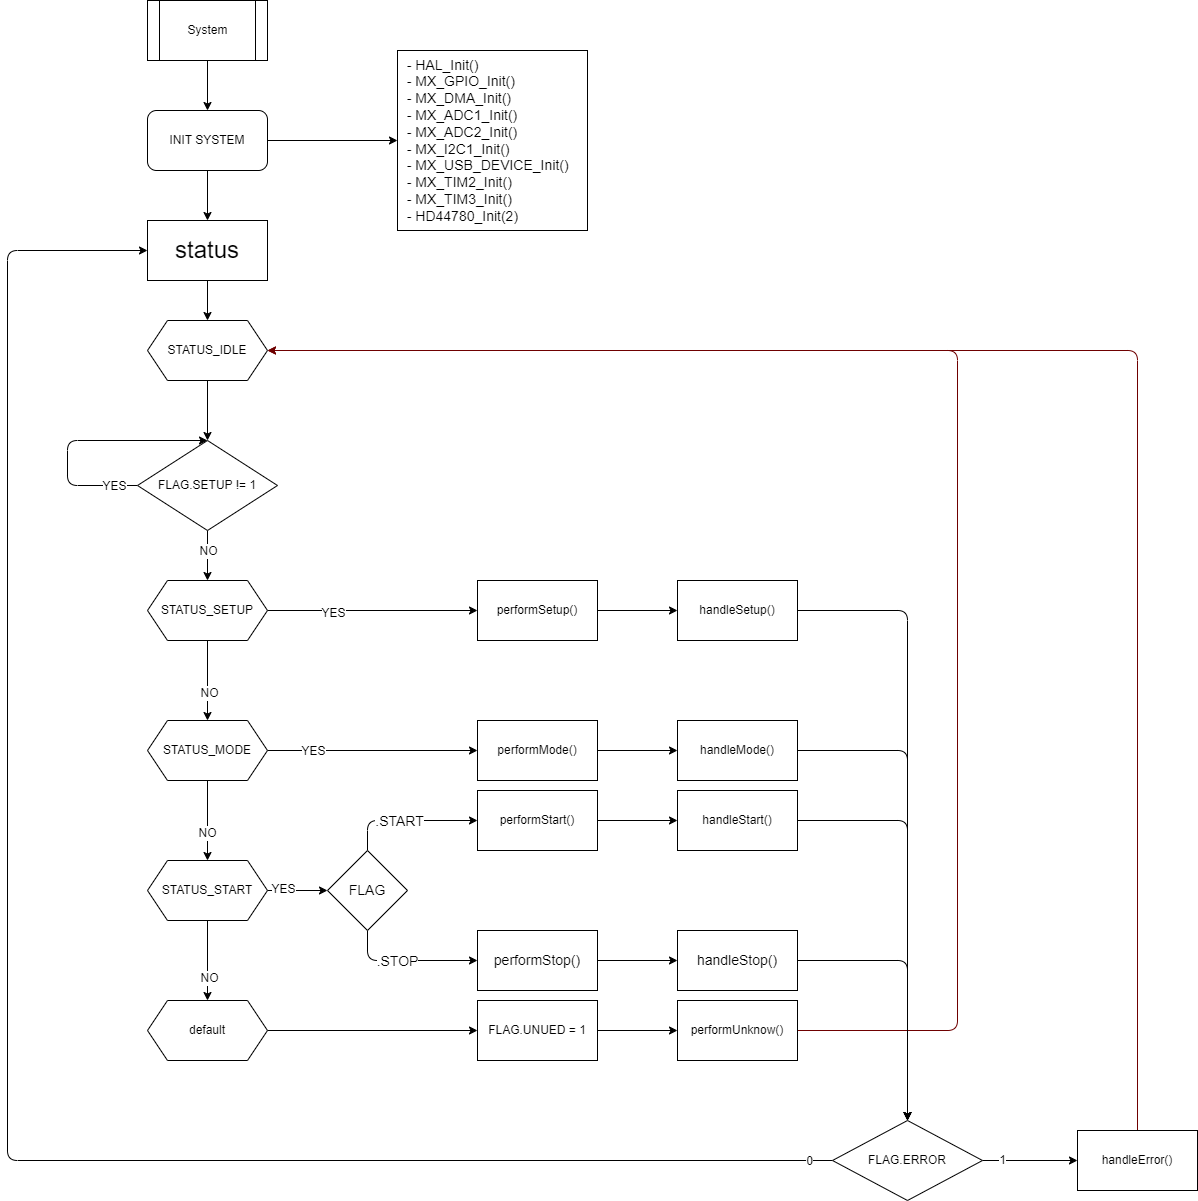
\includegraphics[width=\linewidth]{./diagram/main.png}
	\caption{Sơ đồ hoạt động chính hệ thống}
	\label{f_main system}
\end{figure}

Sau khi xác thực được trạng thái \texttt{status} hệ thống thì vào hàm main tiến hàng xử lý các thao tác vụ của trạng thái đó:

\begin{itemize}[label = -]
	\item \texttt{STATUS\_IDLE}: là trạng thái khởi động của hệ thống hoặc là trạng thái khi hệ thống có xuất hiện lỗi. Có hai lỗi chính của hệ thống là:
		\begin{itemize}[label=+]
			\item Lỗi không nhận diện được MODE của hệ thống: \texttt{FLAG.AC} và \texttt{FLAG.DC} cùng có một giá trị.
			\item Lỗi không nhận diện được START/STOP của hệ thống: \texttt{FLAG.START} và \texttt{FLAG.STOP} có cùng giá trị.
			\item \texttt{handleError()}: là hàm xử lý và hiển thị khi hệ thống xuất hiện lỗi.
		\end{itemize}
	\item \texttt{STATUS\_SETUP}:
		\begin{itemize}[label = +]
			\item \texttt{performSetup()}: là hàm hiển thị lên LCD thể hiện hệ thống đang trong quá trình xử lý khi vào trạng thái SETUP hệ thống.
			\item \texttt{handleSetup()}: là hàm xử lý chính trong khi vào trạng thái SETUP của hệ thống.
		\end{itemize}
	\item \texttt{STATUS\_MODE}:
		\begin{itemize}[label = +]
			\item \texttt{performMode()}: là hàm hiển thị lên LCD thể hiện hệ thống đang trong quá trình xử lý khi vào trạng thái MODE của hệ thống. Thể hiện là hệ thống sẽ hoạt động ở chế độ AC/DC và tầm đo của hệ thống.
			\item \texttt{handleMode()}: là hàm xử lý chính trong khi vào trạng thái MODE của hệ thống.
		\end{itemize}
	\item \texttt{STATUS\_START}: bao gồm hai trạng thái hoạt động là START và STOP.
		\begin{itemize}[label = +]
			\item \texttt{performStart()}/\texttt{performStop()}: là hàm hiển thị lên LCD thể hiện hệ thống đang tiếp tục hay là dừng.
			\item \texttt{handleStart()}/\texttt{handleStop()}: là hàm xử lý chính trong khi vào trạng thái START/STOP của hệ thống.
		\end{itemize}
\end{itemize}

\subsection{Các hàm hoạt động trong ngắt}

\begin{figure}[H]
	\centering
	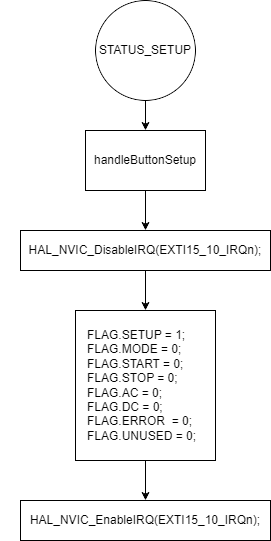
\includegraphics[width=0.5\linewidth]{./diagram/handleButtonSetup.png}
	\caption{HandleButtonSetup}
	\label{f_handlebuttonsetup}
\end{figure}

Hàm \texttt{HandleButtonSetup()} là hàm xử lý trong ngắt, khi có xuất hiện ngắt ở nút nhấn SETUP thì hệ thống sẽ đưa vào trạng thái \texttt{STATUS\_SETUP}, và tiến hành đứa các \texttt{FLAG} và trạng thái ban đầu và bật \texttt{FLAG.SETUP} lên để hệ thống bắt.

\begin{figure}[H]
	\centering
	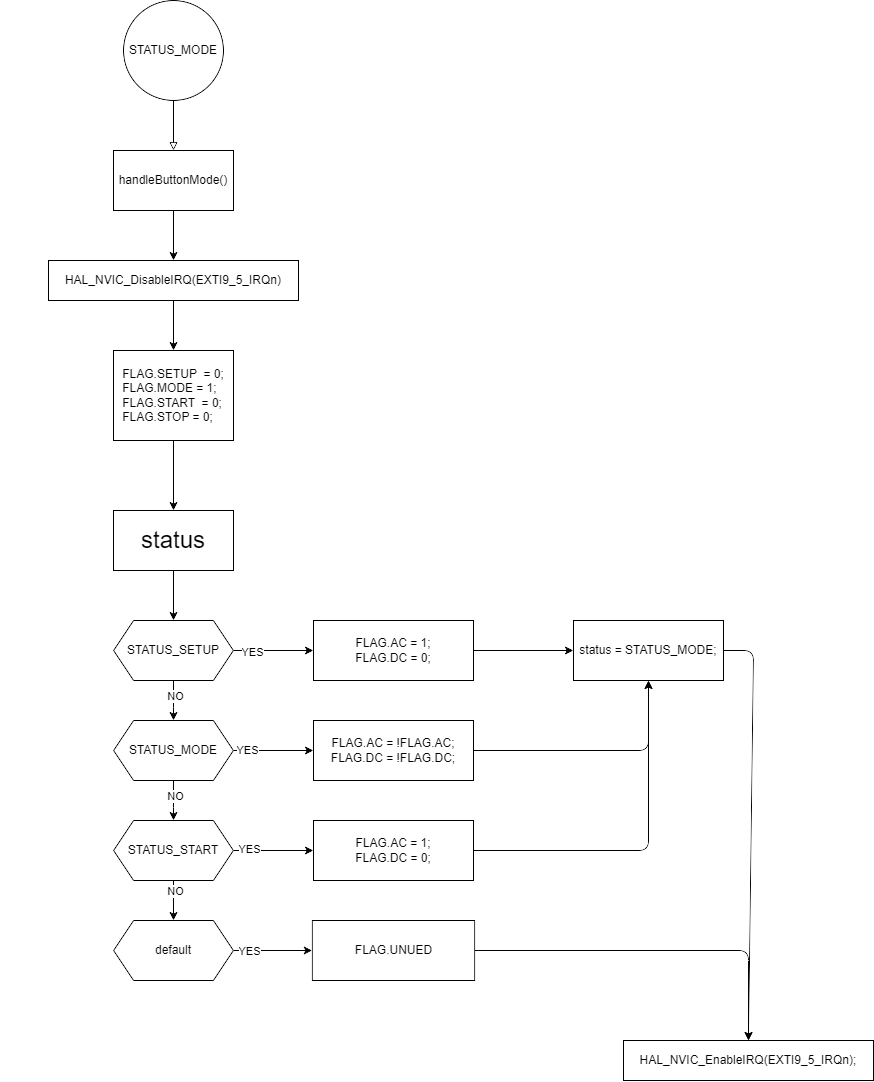
\includegraphics[width=\linewidth]{./diagram/handleButtonMode.png}
	\caption{HandleButtonMode}
	\label{f_handlebuttonmode}
\end{figure}

Hàm \texttt{HandleButtonMode()} là hàm xử lý trong ngắt khi có xuất hiện ngắt ở nút nhấn MODE thì hệ thống sẽ vào kiểm tra các trạng thái trước đó của \texttt{status} về \texttt{STATUS\_MODE} để tiến hành xử lý. Khi \texttt{status} trước đó ở các trạng thái:

\begin{itemize}[label = -]
	\item \texttt{STATUS\_SETUP}: sau khi nhấn nút SETUP thì hệ thống sẽ bật \texttt{FLAG.AC = 1} và \texttt{FLAG.DC = 0} là trạng thái ban đầu sau khi từ trạng thái SETUP qua.
	\item \texttt{STATUS\_MODE}: khi tiếp tục nhấn nút MODE thì hệ thống sẽ tự động tráo đổi giá trị của các \texttt{FLAG.AC} và \texttt{FLAG.DC}.
	\item \texttt{STATUS\_START}: khi nhấn nút MODE trong khi hệ thống đang hoạt động để cài đặt lại chế độ cho hệ thống.
\end{itemize}

\begin{figure}[H]
	\centering
	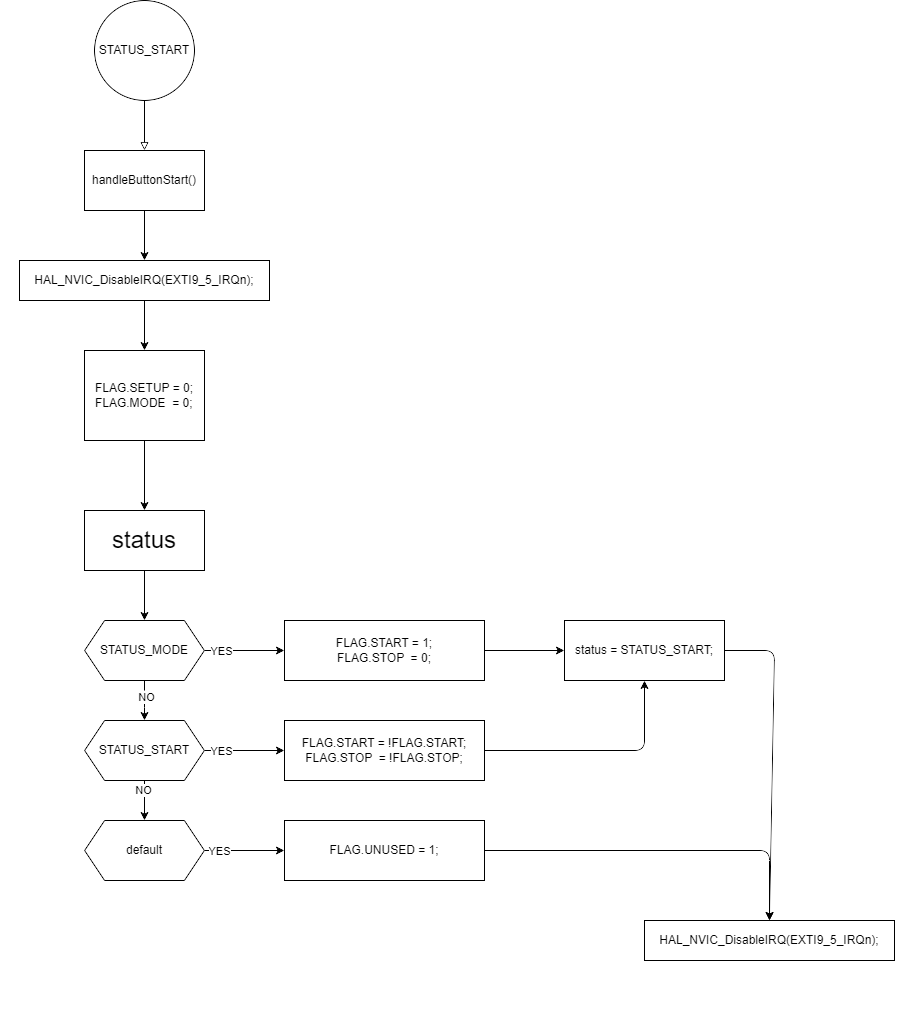
\includegraphics[width=\linewidth]{./diagram/handleButtonStart.png}
	\caption{HandleButtonStart}
	\label{f_handlebuttonstart}
\end{figure}

Hàm \texttt{HandleButtonStart()} là hàm xử lý trong ngắt khi có xuất hiện ngắt ở nút nhấn START/STOP thì hệ thống sẽ vào kiểm tra các trạng thái trước đó của \texttt{status} và trả về trạng thái \texttt{STATUS\_START} để tiến hành xử lý. Khi \texttt{status} trước đó ở các trạng thái:

\begin{itemize}[label = -]
	\item \texttt{STATUS\_MODE}: sau khi đã cài đặt xong chế độ ở MODE thì hệ thống sẽ bật \texttt{FLAG.START = 1} và \texttt{FLAG.STOP = 0} để đưa hệ thống vào trạng thái hoạt động START.
	\item \texttt{STATUS\_START}: khi nhấn nhấn nút START/STOP để đổi trạng thái START và STOP hệ thống bằng các thay đổi hai giá trị \texttt{FLAG.START} và \texttt{FLAG.STOP} với nhau.
\end{itemize}

\subsection{Các hàm hoạt động xử lý trong main}

\begin{figure}[H]
	\centering
	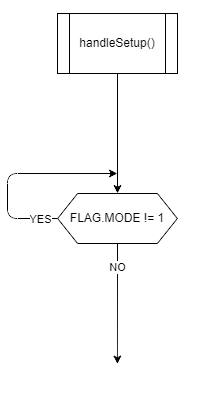
\includegraphics[width=0.3\linewidth]{./diagram/handleSetup.png}
	\caption{HandleSetup}
	\label{f_handlesetup}
\end{figure}

Hàm \texttt{HandleSetup()} là hàm xử lý trong chế độ SETUP, hệ thống sẽ hoạt động động chỉ khi có tín hiệu kích hoạt của \texttt{FLAG.MODE} tức khi đã nhấn nút SETUP thì tiếp theo chỉ có thể nhấn nút MODE để hệ thống hoạt động.

\begin{figure}[H]
	\centering
	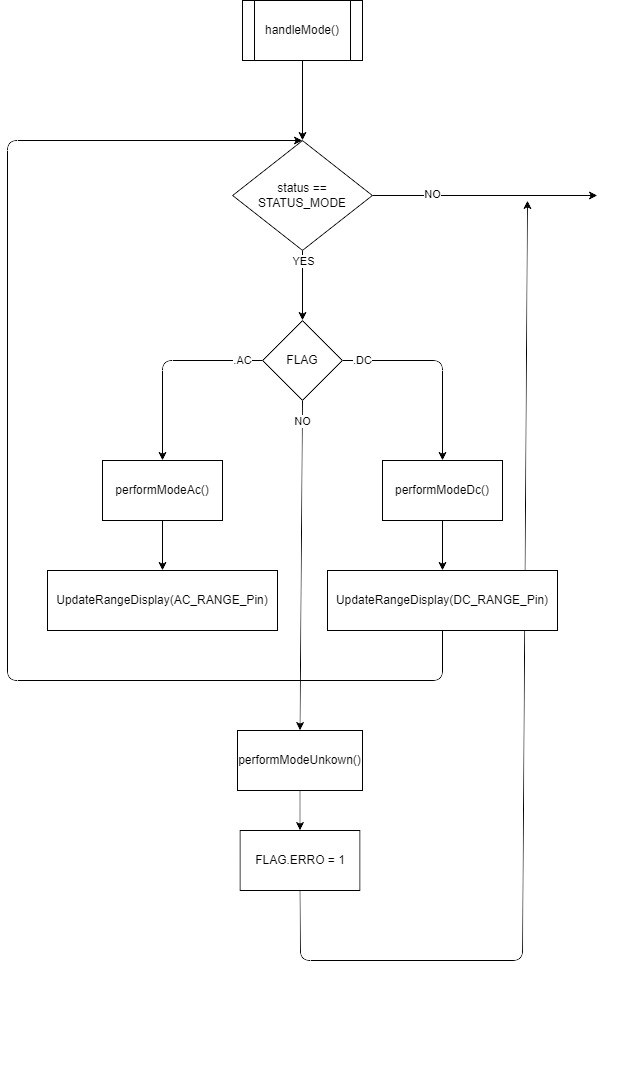
\includegraphics[width=0.7\linewidth]{./diagram/handleMode.png}
	\caption{HandleMode}
	\label{f_handlemode}
\end{figure}

Hàm \texttt{HandleMode()} là hàm xử lý trong chế độ MODE, hệ thống thực hiện các bước sau:

\begin{enumerate}[label=Bước \arabic *:]
	\item Kiểm tra xem có còn đang ở trong trạng thái \texttt{STATUS\_MODE} hay không. Nếu vẫn là ở trạng thái \texttt{STATUS\_MODE} thì tiếp tục nếu không thì thoát khỏi hàm.
	\item Kiểm tra \texttt{FLAG} xem đang hoạt động ở chế độ AC hay DC nếu không thuộc hai chế độ trên thì hệ thống sẽ nhận diện được lỗi và sử dụng hàm \texttt{performModeUnkown()} để thể hiện cho người dùng biết là có lỗi không nhận diện được chế độ hoạt của hệ thống.
		\begin{itemize}[label=-]
			\item \texttt{FLAG.AC}:
				\begin{itemize}[label = +]
					\item Đầu tiên là xử lý hàm \texttt{performModeAC()} để hiển thị cho người dùng biết là đang cài đặt chế độ AC.
					\item Tiếp là là hàm \texttt{UpdateRangeDisplay(AC\_RANGE\_Pin)} để nhận biết được tầm đo của hệ thống.					
				\end{itemize}
			\item \texttt{FLAG.DC}:
				\begin{itemize}[label = +]
					\item Đầu tiên là xử lý hàm \texttt{performDC()} để hiện thị cho người dùng biết là đang cài đặt chế độ DC.
					\item Tiếp là là hàm \texttt{UpdateRangeDisplay(DC\_RANGE\_Pin)} để nhận biết được tầm đo của hệ thống.
				\end{itemize}
		\end{itemize}
\end{enumerate}

\begin{figure}[H]
	\centering
	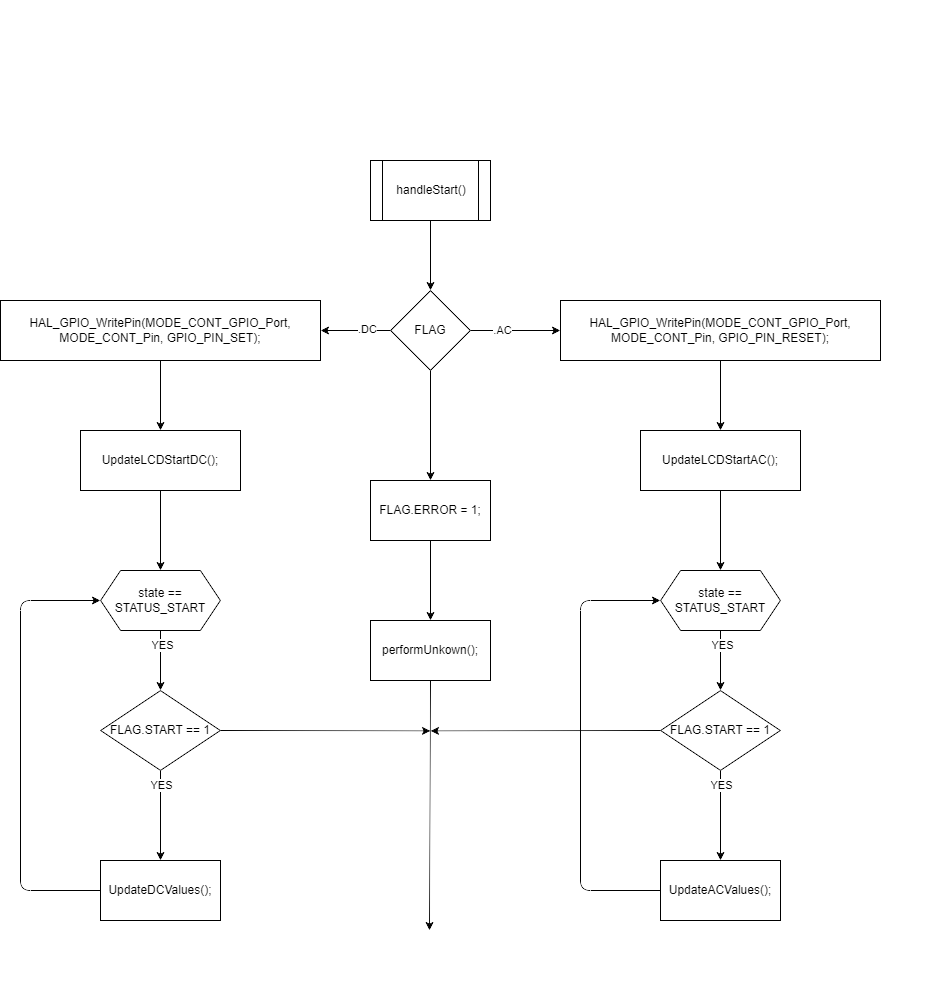
\includegraphics[width=\linewidth]{./diagram/handleStart.png}
	\caption{HandleStart}
	\label{f_handlestart}
\end{figure}

Hàm \texttt{HandleStart()} là hàm xử lý khi hệ thống ở chế độ hoạt động, hệ thống sẽ thực hiện các hàm sau đây:

\begin{enumerate}[label = Bước \arabic *:]
	\item Kiểm tra \texttt{FLAG} xem hệ thống đang hoạt động ở chế độ AC hay DC, nếu không thuộc hai chế trên thì hệ thống nhận diện được lỗi và thực hiện hàm \texttt{performUnkown()} để thể hiện cho người dùng biết được xuất hiện lỗi không nhận diện được chế độ hoạt động.
	\item Nếu ở chế độ AC thì RESET tín hiệu chân điều khiển Relay để hoạt động chế độ đo AC, còn nếu là ở chế độ DC thì SET tín hiệu chân điều khiển Relay hoạt động để hoạt động chế độ đo DC.
	\item Sau khi đã cài đặt chế độ cho Relay, thì thực hiện hàm \texttt{UpdateLCDStartDC()} hoặc \texttt{UpdateLCDStartAC()} để hiển thị các giá trị cần hiển thị lên LCD ở mỗi chế độ.
		\begin{itemize}[label=-]
			\item Với chế độ DC thì hiển thị giá trị điện áp \texttt{VALUE.VDC}.
			\item Với chế độ AC thì hiển thị giá trị điệp áp đỉnh đỉnh \texttt{VALUE.VPP} và giá trị tần số \texttt{VALUE.FREQ}.
		\end{itemize}
	\item Kiểm tra trạng thái xem vẫn ở trạng thái \texttt{STATUS\_START} hay không và xem \texttt{FLAG.START} có bật để tiếp tục thực hiện, nếu không thỏa thì phải thoát khỏi hàm để xử lý các hàm tiếp theo.
	\item Hiển thị giá trị đo được của hệ thống trả về cho từng chế độ.
		\begin{itemize}[label = -]
			\item Với chế độ DC thì sử dụng hàm \texttt{UpdateDCValue()} để xuất giá trị điện áp DC lên LCD.
			\item Với chế độ AC thì sử dụng hàm \texttt{UpdateACValue()} để xuất giá trị điện áp đỉnh đỉnh và tần số lên LCD.
		\end{itemize}
\end{enumerate}

\begin{figure}[H]
	\centering
	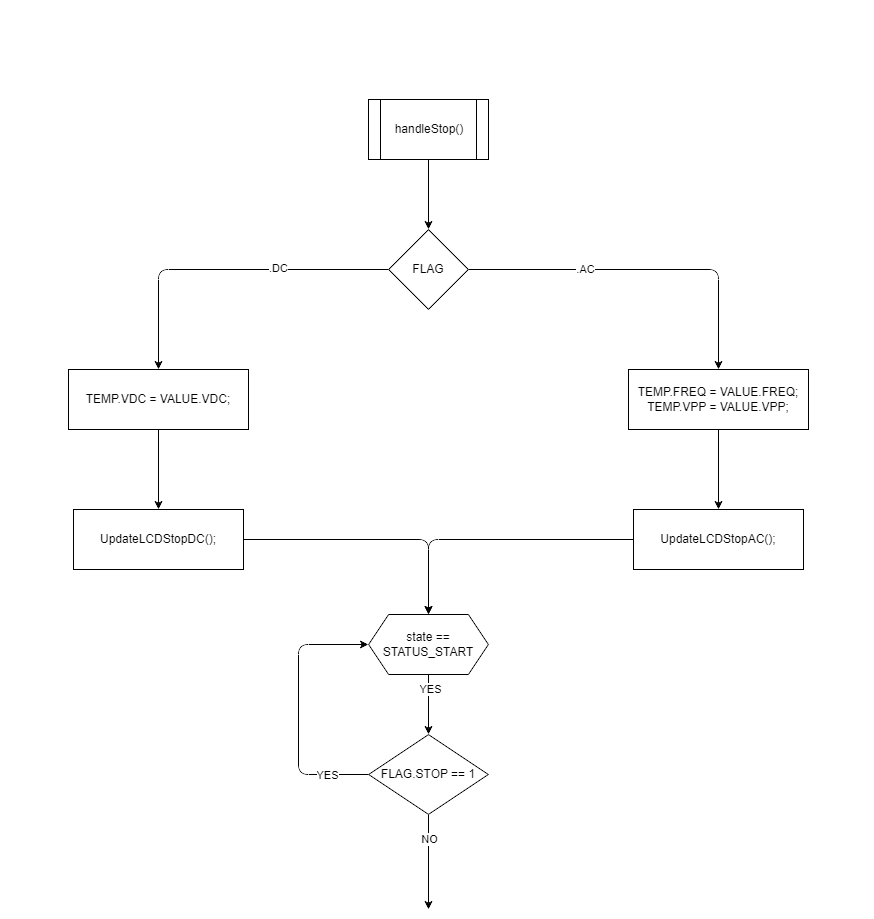
\includegraphics[width=\linewidth]{./diagram/handleStop.png}
	\caption{HandleStop}
	\label{f_handlestop}
\end{figure}

Hàm \texttt{HandleStop()} là hàm xử lý khi hệ thống tạm dừng, hệ thống sẽ thực hiện các bước sau đây:

\begin{enumerate}[label = Bước \arabic *:]
	\item Kiểm tra \texttt{FLAG} xem hệ thống hoạt động ở chế độ AC hay DC.
	\item Thực hiện các bước sau:
		\begin{itemize}[label = -]
			\item Nếu ở chế độ AC:
				\begin{itemize}[label = +]
					\item Gán giá trị \texttt{VALUE.VPP} và \texttt{VALUE.FREQ} vào các biến lưu trữ tạm khi vào chế độ dừng hiển thị.
					\item Sử dụng hàm \texttt{UpdateLCDStopAC()} để hiển thị các giá trị trước khi vào chế độ STOP để cho phép người dùng dễ dàng theo dõi giá trị đó.
				\end{itemize}
			\item Nếu ở chế độ DC:
				\begin{itemize}[label = +]
					\item Gán giá trị \texttt{VALUE.VDC} vào biến lưu trữ tạm khi vào chế độ dừng hiển thị.
					\item Sử dụng hàm \texttt{UpdateLCDStopDC()} để hiển thị các giá trị trước khi vào chế độ STOP để cho phép người dùng dễ dàng theo dõi giá trị đó.
				\end{itemize}
		\end{itemize}
	\item Kiểm tra nếu vẫn ở trạng thái \texttt{STATUS\_START} và \texttt{FLAG.STOP} thì vẫn treo chương trình cho đến khi có tín hiệu thay đổi trạng thái.
\end{enumerate}
\section{Software}

\begin{figure}[H]
	\centering
	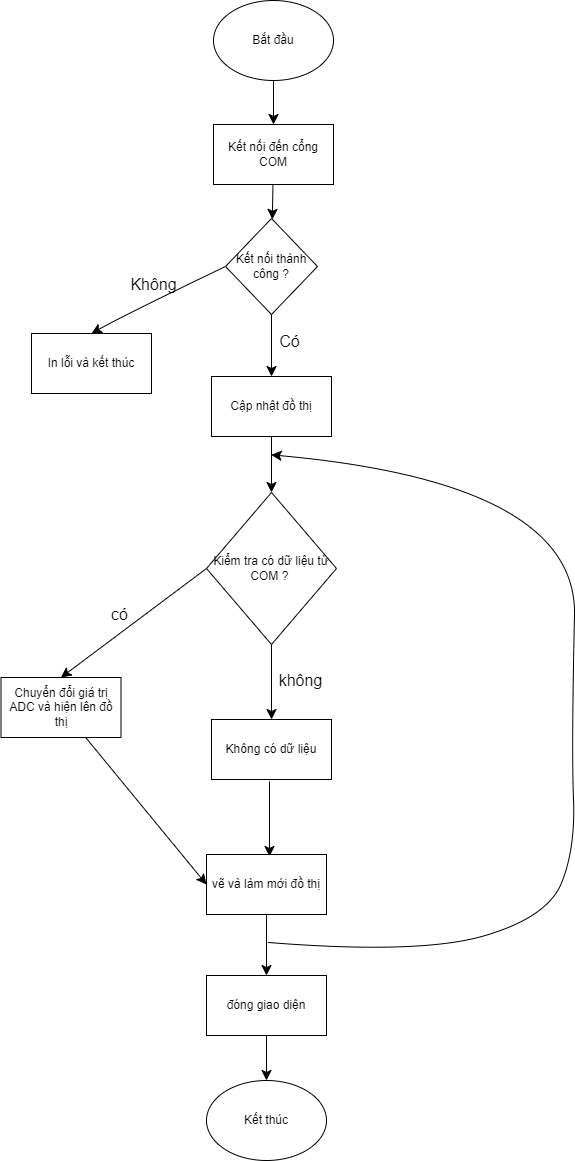
\includegraphics[width=0.6\linewidth]{./diagram/software_diagram.drawio.png}
	\caption{Lưu đồ đọc giá trị điện áp từ dữ liệu serial port}
	\label{f_luu do doc gia tri dien ap tu du lieu serial port}
\end{figure}

\begin{enumerate}[label = Bước \arabic *:]
	\item Bắt đầu chương trình: khởi tạo các biến kết nối đến cổng COM.
	\item Kết nối đến cổng COM:
		\begin{itemize}[label=-]
			\item Input: \texttt{PORT}, \texttt{BAUD\_RATE}.
			\item Kiểm tra kết nối serial: 
				\begin{itemize}[label = +]
					\item Nếu thành công: Trả về đối tượng ser.
					\item Nếu thất bại: In thông báo lỗi và kết thúc kết nối.
				\end{itemize}
		\end{itemize}
	\item Cập nhật đồ thị: kiểm tra dữ liệu từ cổng COM:
		\begin{itemize}[label = -]
			\item Nếu có dữ liệu, đọc chuỗi và kiểm tra định dạng 'ADC Value'. Lọc giá trị ADC từ chuỗi, và chuyển đổi giá trị ADC thành giá trị điện áp. Cập nhật dữ liệu thời gian (x\_data) và điện áp (y\_data). Làm mới đồ thị với dữ liệu mới.
			\item Nếu không có dữ liệu thì làm mới đồ thị.
		\end{itemize}
	\item Giao diện Tkinter:
		\begin{itemize}[label=-]
			\item Khởi tạo cửa sổ giao diện chính.
			\item Vẽ khung đồ thị bằng Matplotlib.
			\item Gán hàm cập nhật đồ thị vào sự kiện định kỳ (after(100)).
		\end{itemize}
	\item Vòng lặp giao diện: chạy vòng lặp chính của Tkinter (mainloop()). Kết thúc thì người dùng đóng ứng dụng để thoát chương trình.
\end{enumerate}